% !TEX root = Assignment_3_Solution.tex
% Format based on the Assignment Homework Solutions Template.
\documentclass[a4paper,11pt]{article}
\usepackage{comment}
\usepackage{lipsum}
\usepackage{fullpage}
\usepackage{verbatim}
\usepackage{graphicx}
\usepackage{amsmath}
\usepackage{amssymb,amsthm}
\usepackage{tikz}
\usetikzlibrary{arrows,positioning}
\usepackage{xcolor}
\usepackage{booktabs}
\usepackage{array}
\usepackage{listings}
\usepackage{float}
\usepackage{mdframed}
\usepackage[shortlabels]{enumitem}
\usepackage{indentfirst}
\usepackage{hyperref}
\usepackage{placeins}
\usepackage{caption}
\usepackage{needspace}

\newenvironment{problem}[1]
    {\begin{mdframed}[backgroundcolor=gray!20]\textbf{Problem #1}\\}
    {\end{mdframed}}
\newenvironment{solution}{\textit{Solution:}}{}
\newcommand{\ones}{\mathbf{1}}
\newcommand{\R}{\mathbb{R}}
\newcommand{\N}{\mathbb{N}}
\newcommand{\argmin}{\operatorname*{arg\,min}}
\newcommand{\norm}[1]{\left\|#1\right\|}
\lstset{language=Python,basicstyle=\ttfamily\scriptsize,breaklines=true,frame=single,
  columns=fullflexible,keepspaces=true,showstringspaces=false}
\hypersetup{colorlinks=true,linkcolor=blue!50!black,urlcolor=blue!50!black}
\setlength{\tabcolsep}{4pt}
\renewcommand{\arraystretch}{1.15}
\setlength{\parskip}{0.35em}
\emergencystretch=2em
\setcounter{MaxMatrixCols}{20}

\begin{document}

\noindent
\large\textbf{Dhruv Goyal} \hfill \textbf{Assignment-\#3}\\[2pt]
ID: \texttt{EP23BTECH11008} \hfill Submission Date: 18 September 2026\\[1pt]
\normalsize Course: AI3403-Multi-Agent Systems\\[1pt]
Instructor: Dr. Venkatraman Renganathan\\
\noindent\rule{\textwidth}{2.8pt}

\begin{problem}{1}
Fix the number of agents to be $N = 20$. Generate a connected graph using Erdos-Renyi model for
$N$ agents and some $p \in (0, 1)$. Assume random initial positions for all $N$ agents in $\R^2$.
Using formation control strategy, display your name in capital letters in $\R^2$, letter by letter
in a sequence. For instance, my name is Venkat and this is how I would do:
\begin{itemize}
\item Starting from initial position vector $x[0]$, agents should go to positions forming the letter V.
\item Starting from positions corresponding to letter V, agents should go to positions corresponding
to letter E.
\item Continue this letter sequence, until agents go to letter T.
\end{itemize}
Record your name formation sequence as an animation video through your simulation, host it in your
github and simply give just the Github link containing both the code and the video as your solution.
Ensure that your Github repository is made public before submitting. For people having big lengthy
names, choose the corresponding name which people use to call you on a regular basis - not the full
entire name. For instance, if a student's full name is Manoj Kumar Sahu, and he goes commonly by
simply Manoj, then he should simulate the sequence MANOJ.
\end{problem}

\begin{solution}
I use the name \textbf{DHRUV}, which is the short name used regularly. There are $N=20$ agents,
unit edge weights, and a connected $G(20,0.25)$ graph. The graph was generated with seed
$20260905$; the first connected graph was used, so no edges were added by hand.

\textbf{Notation note.} The question calls the initial stacked position $x[0]$. In the solution I
use $p_i[k]$ for the position of agent $i$ and $p[k]$ for the stacked position, so the question's
$x[0]$ is the same as $p[0]$ here.

For agent $i$, let $p_i[k]\in\R^2$ be its position and let $r_i^{(\ell)}\in\R^2$ be its target
point for letter $\ell$. I apply consensus to the translated positions:
\[
z_i[k]=p_i[k]-r_i^{(\ell)},\qquad
u_i[k]=\sum_{j\in\mathcal N_i}\left((p_j[k]-p_i[k])-(r_j^{(\ell)}-r_i^{(\ell)})\right).
\]
With $p[k]$ and $r^{(\ell)}$ stacked in $\R^{40}$, the update is
\[
\boxed{p[k+1]=p[k]-\Delta t(L\otimes I_2)(p[k]-r^{(\ell)})},
\qquad L=D-A.
\]
In simple terms: subtracting the desired points makes ordinary consensus produce the required
relative shape.

Each capital letter is drawn from line segments in the same $[-2.5,2.5]\times[-3,3]$ frame.
Exactly 20 points are sampled by arc length and the mean point is subtracted, so every letter has
the same centre. The initial positions are sampled uniformly from $[-5,5]\times[-4,4]$. The final
positions of one letter are used as the initial positions for the next letter.

The resulting formation-offset matrices are listed below. Entries are rounded to three decimals;
the simulation uses the full-precision values returned by the code.
\[
\begin{array}{c@{\qquad}c@{\qquad}c}
R^{(D)}=\left[\begin{smallmatrix}
-1.489&-2.841\\-1.489&-1.914\\-1.489&-0.986\\-1.489&-0.059\\-1.489&0.869\\
-1.489&1.797\\-1.489&2.724\\-0.996&3.159\\-0.068&3.159\\0.813&2.986\\
1.619&2.525\\1.911&1.767\\1.911&0.839\\1.911&-0.088\\1.911&-1.016\\
1.911&-1.943\\1.190&-2.453\\0.366&-2.841\\-0.562&-2.841\\-1.489&-2.841
\end{smallmatrix}\right]&
R^{(H)}=\left[\begin{smallmatrix}
-2.185&-2.700\\-2.185&-1.950\\-2.185&-1.200\\-2.185&-0.450\\-2.185&0.300\\
-2.185&1.050\\-2.185&1.800\\-2.185&2.550\\2.415&-2.700\\2.415&-1.843\\
2.415&-0.986\\2.415&-0.129\\2.415&0.729\\2.415&1.586\\2.415&2.443\\
-2.185&0.300\\-1.035&0.300\\0.115&0.300\\1.265&0.300\\2.415&0.300
\end{smallmatrix}\right]&
R^{(R)}=\left[\begin{smallmatrix}
-1.507&-3.341\\-1.507&-2.459\\-1.507&-1.576\\-1.507&-0.694\\-1.507&0.189\\
-1.507&1.071\\-1.507&1.953\\-1.330&2.659\\-0.447&2.659\\0.435&2.659\\
1.173&2.224\\1.740&1.666\\1.303&0.900\\0.865&0.134\\0.258&-0.341\\
-0.624&-0.341\\0.593&-0.341\\1.393&-1.341\\2.193&-2.341\\2.993&-3.341
\end{smallmatrix}\right]
\end{array}
\]
\[
\begin{array}{c@{\qquad}c}
R^{(U)}=\left[\begin{smallmatrix}
-2.300&3.465\\-2.300&2.649\\-2.300&1.834\\-2.300&1.019\\-2.300&0.203\\
-2.300&-0.612\\-2.300&-1.427\\-1.827&-2.061\\-1.223&-2.535\\-0.408&-2.535\\
0.408&-2.535\\1.223&-2.535\\1.827&-2.061\\2.300&-1.427\\2.300&-0.612\\
2.300&0.203\\2.300&1.019\\2.300&1.834\\2.300&2.649\\2.300&3.465
\end{smallmatrix}\right]&
R^{(V)}=\left[\begin{smallmatrix}
-2.400&2.842\\-2.147&2.211\\-1.895&1.579\\-1.642&0.947\\-1.389&0.316\\
-1.137&-0.316\\-0.884&-0.947\\-0.632&-1.579\\-0.379&-2.211\\-0.126&-2.842\\
0.126&-2.842\\0.379&-2.211\\0.632&-1.579\\0.884&-0.947\\1.137&-0.316\\
1.389&0.316\\1.642&0.947\\1.895&1.579\\2.147&2.211\\2.400&2.842
\end{smallmatrix}\right]
\end{array}
\]

\begin{figure}[H]
\centering
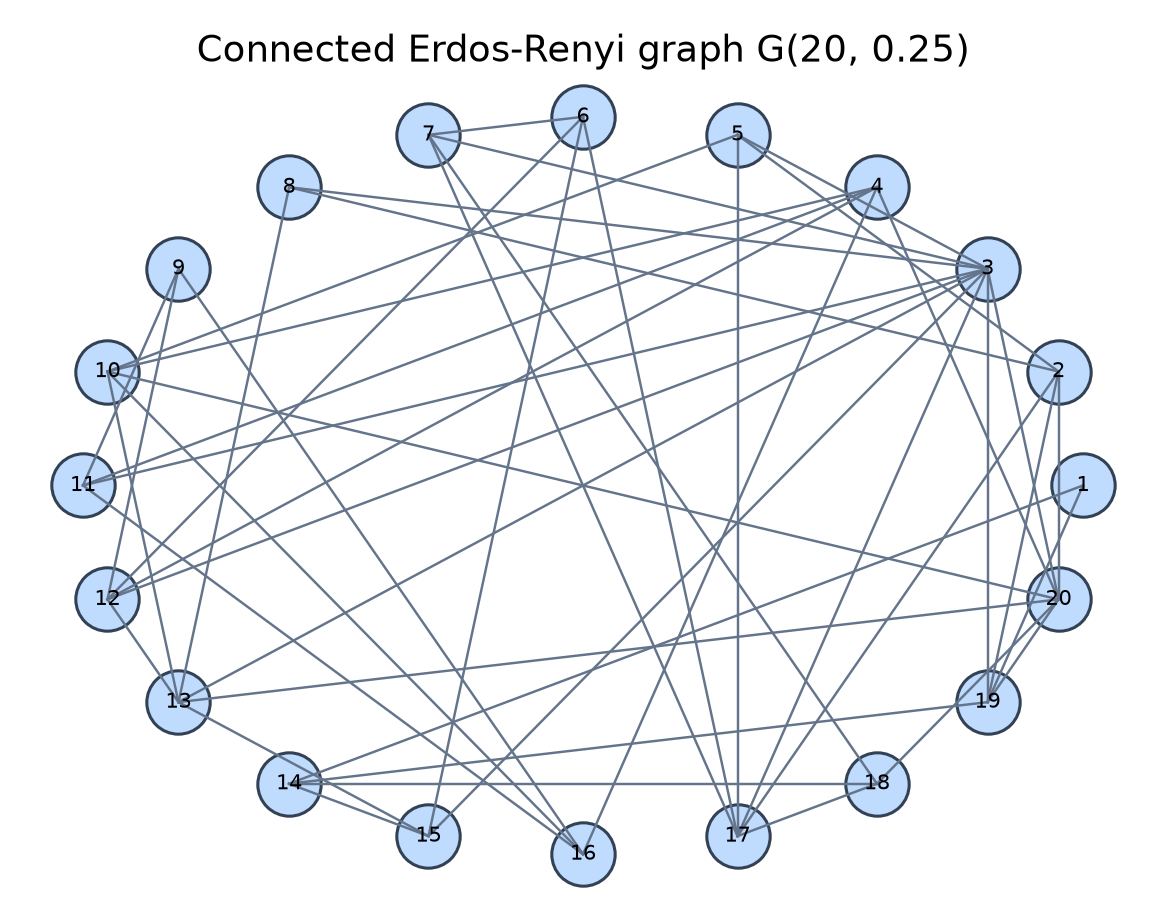
\includegraphics[width=.48\textwidth]{assets/p1_graph.png}
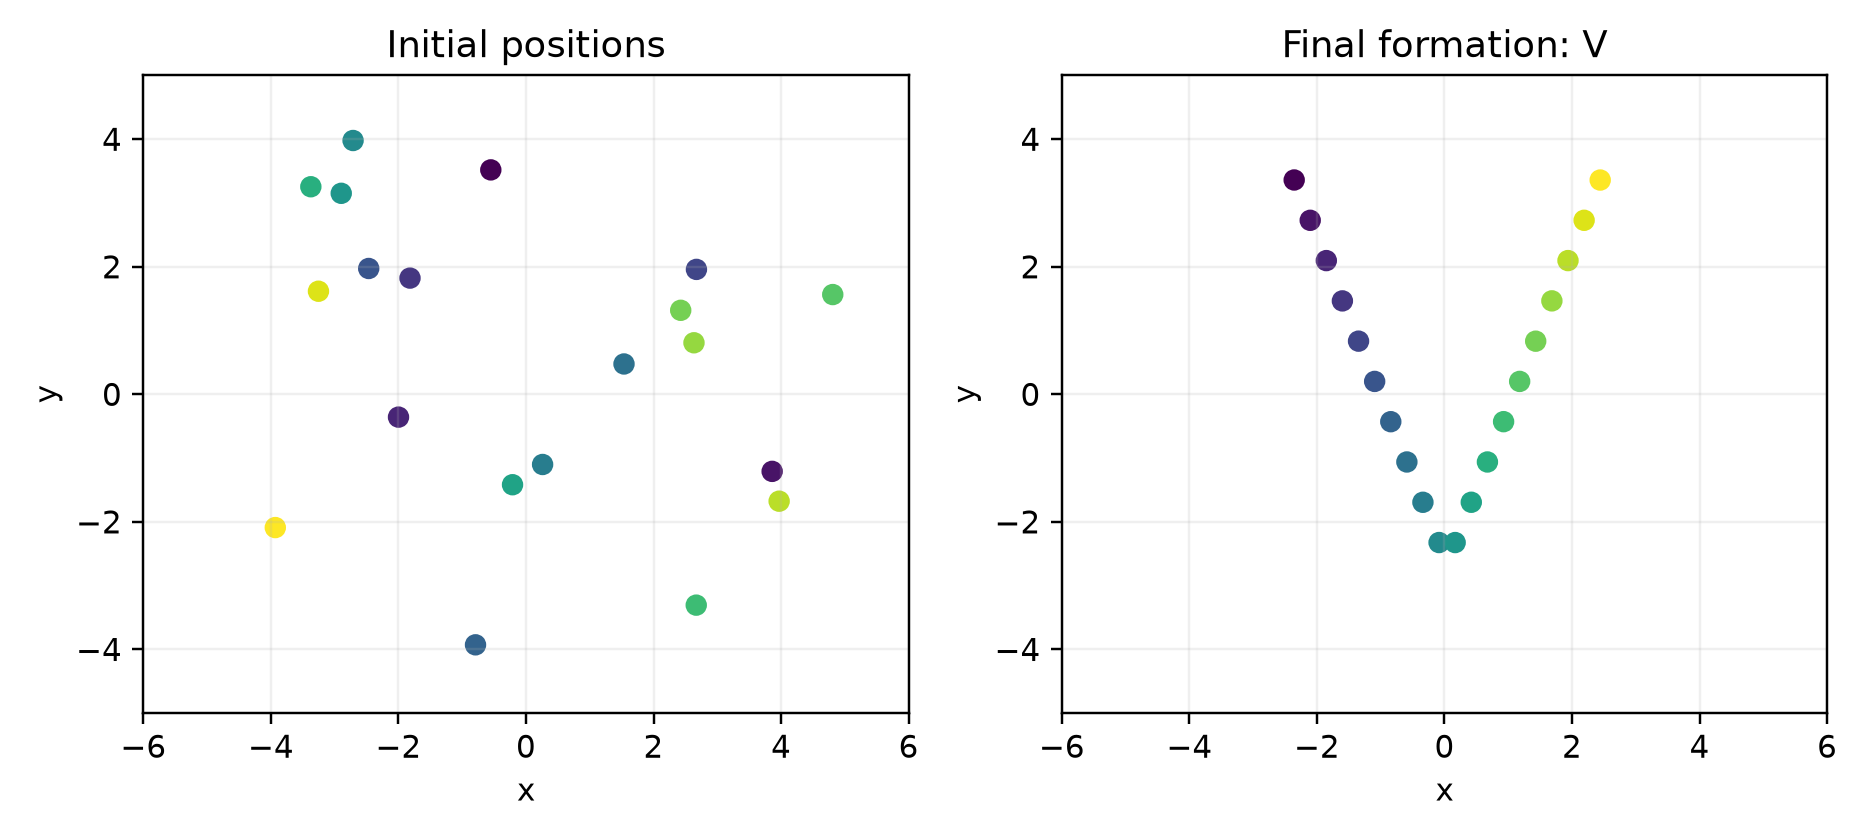
\includegraphics[width=.48\textwidth]{assets/p1_initial_final.png}
\caption{The connected communication graph, the random initial cloud, and the final V formation.}
\end{figure}

The graph has $\lambda_2(L)=0.910671>0$, so it has exactly one zero Laplacian eigenvalue and is
connected. The largest Laplacian eigenvalue is $\lambda_{\max}(L)=11.496026$. I use
$\Delta t=0.12$, which satisfies $0<0.12<2/\lambda_{\max}=0.173973$. The stopping value is
\[
\varepsilon_{\mathrm{form}}[k]=\max_{(i,j)\in E}
\left\|(p_i[k]-p_j[k])-(r_i^{(\ell)}-r_j^{(\ell)})\right\|,
\]
with tolerance $10^{-3}$. The final edge errors for D, H, R, U, and V are respectively
$9.41\times10^{-4}$, $9.87\times10^{-4}$, $9.93\times10^{-4}$,
$9.32\times10^{-4}$, and $9.43\times10^{-4}$.

\begin{figure}[H]
\centering
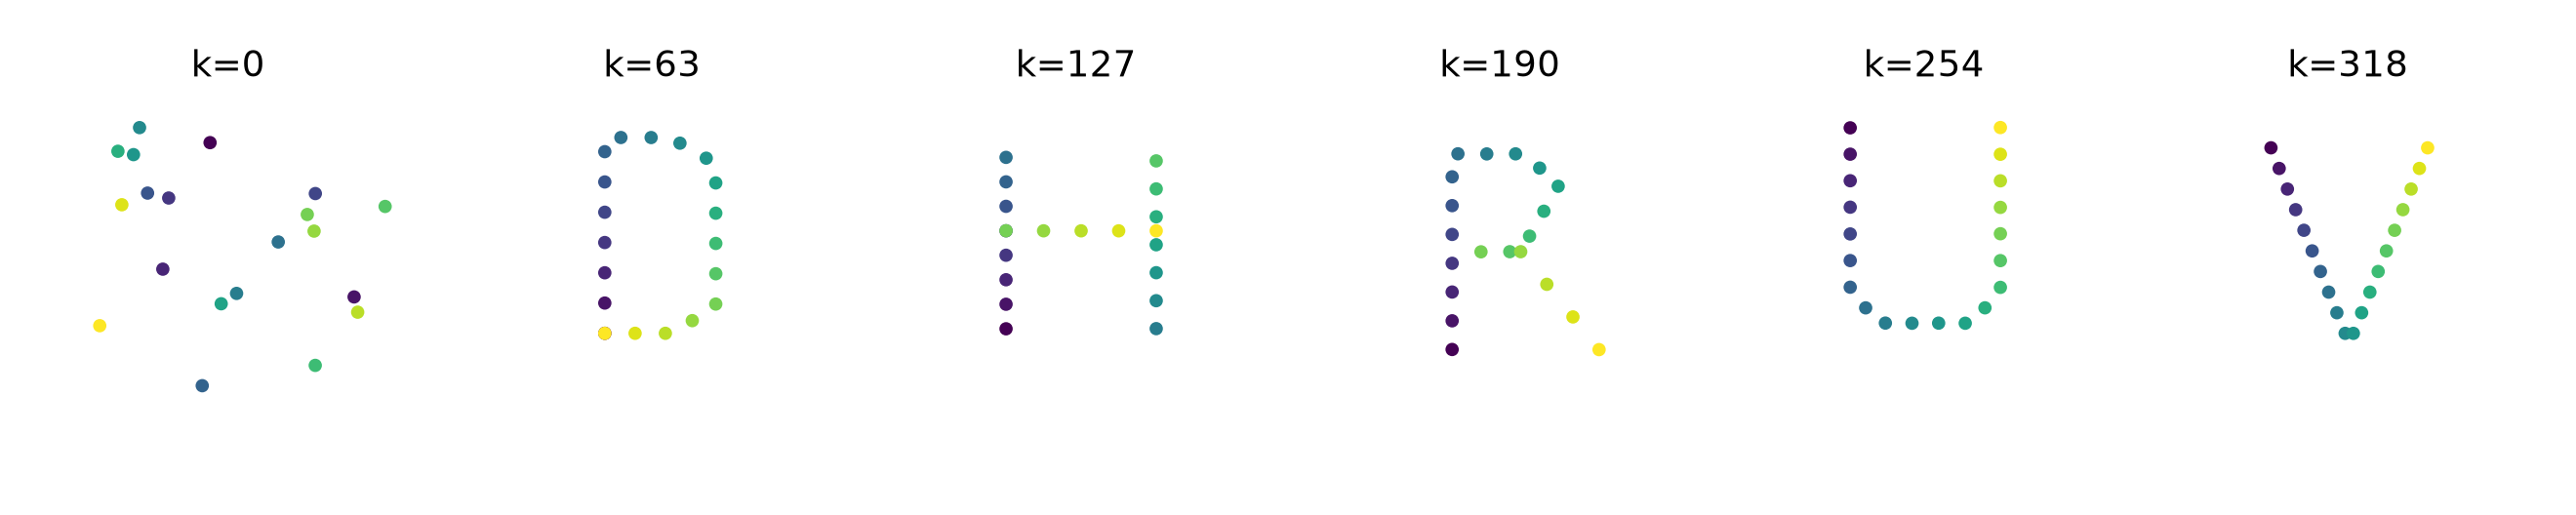
\includegraphics[width=.98\textwidth]{assets/p1_frame_strip.png}
\caption{Selected fixed-axis frames from the DHRUV formation sequence.}
\end{figure}

The animation file is \texttt{assets/p1\_DHRUV\_formation.gif}, and the source code is included below.
The code appendix is included because the submission rules require code in the PDF. The required
public GitHub repository containing both the code and the animation is:
\begin{center}
\fbox{\parbox{0.82\textwidth}{\centering\textbf{Public GitHub repository (Problem 1):}\\
\url{https://github.com/splittersplatter/MAS}}}
\end{center}

\subsection*{Graph matrices}
Rows and columns use the order $1,2,\ldots,20$. The adjacency matrix has $a_{ij}=1$ exactly when
agents $i$ and $j$ communicate, and $a_{ii}=0$.
\[
{\scriptstyle A=\begin{bmatrix}
0&0&0&0&0&0&0&0&0&0&0&0&0&1&0&0&0&0&1&0\\
0&0&0&0&1&0&0&1&0&0&0&0&0&0&0&0&1&0&1&1\\
0&0&0&0&1&0&1&1&0&0&1&1&1&0&1&0&1&0&1&1\\
0&0&0&0&0&0&0&0&0&1&1&1&0&0&0&1&0&0&0&1\\
0&1&1&0&0&0&0&0&0&1&0&0&0&0&0&0&1&0&0&0\\
0&0&0&0&0&0&1&0&0&0&0&1&0&0&1&0&1&0&0&0\\
0&0&1&0&0&1&0&0&0&0&0&0&0&0&0&0&1&1&0&0\\
0&1&1&0&0&0&0&0&0&0&0&0&1&0&0&0&0&0&0&0\\
0&0&0&0&0&0&0&0&0&0&1&1&0&0&0&1&0&0&0&0\\
0&0&0&1&1&0&0&0&0&0&0&0&1&0&0&1&0&0&0&1\\
0&0&1&1&0&0&0&0&1&0&0&0&0&0&0&1&0&0&0&0\\
0&0&1&1&0&1&0&0&1&0&0&0&1&0&0&0&0&0&0&0\\
0&0&1&0&0&0&0&1&0&1&0&1&0&0&1&0&0&0&0&1\\
1&0&0&0&0&0&0&0&0&0&0&0&0&0&1&0&0&1&1&0\\
0&0&1&0&0&1&0&0&0&0&0&0&1&1&0&0&0&0&0&0\\
0&0&0&1&0&0&0&0&1&1&1&0&0&0&0&0&0&0&0&0\\
0&1&1&0&1&1&1&0&0&0&0&0&0&0&0&0&0&1&0&0\\
0&0&0&0&0&0&1&0&0&0&0&0&0&1&0&0&1&0&0&1\\
1&1&1&0&0&0&0&0&0&0&0&0&0&1&0&0&0&0&0&1\\
0&1&1&1&0&0&0&0&0&1&0&0&1&0&0&0&0&1&1&0
\end{bmatrix}.}
\]
\[
{\small D=\operatorname{diag}(2,5,10,5,4,4,4,3,3,5,4,5,6,4,4,4,6,4,5,7),}
\qquad L=D-A.
\]
This explicitly defines every entry of $L$ and is less error-prone to read than repeating the same
20 by 20 array. The code below also prints the full numerical $L$ matrix.

\subsection*{Problem 1 code}
\lstinputlisting{Assignment_3_Problem_1.py}
\end{solution}

\clearpage
\begin{problem}{2}
Suppose that there is a target intruder which has to be tracked by a swarm of $N\in\N$ drones.
Each of the $N$ drones are equipped with a sensor and the drones are connected by a communication
network $G(V,E)$. The initial location of the intruder is denoted by $z_0\in\R^3$ is not known
exactly and $z_0\sim\mathcal N(\bar z_0,\Sigma_0)$, where mean $\bar z_0\in\R^3$ and covariance
$\Sigma_0\in\R^{3\times3}$ and is positive semi-definite.

The intruder target is doing a random walk with dynamics given by
\[
z(t+1)=z(t)+w,\quad \forall t\in\N,
\]
where $w\sim\mathcal N(0,\Sigma_w)$ denotes the process noise (like the wind disturbance).
Each sensor $i$ is located at $x_i\in\R^3$ and assume that sensor $i$ mounted on drone $i$ knows
its location $x_i$, and its measurement data $y_i(t)$ is given by the model $\forall t\in\N$ as
\[
y_i(t)=x_i-z(t)+v_i.
\]
Here $v_i$ is a random sensor measurement noise with $v_i\sim\mathcal N(0,\Sigma_v^{(i)})$,
where $\Sigma_v^{(i)}\succeq0$ is also known to agent $i$. We assume that noises for different
sensors are independent. Now let each drone with its respective sensor $i=1,\ldots,N$ take one
measurement using the model and obtain $y_i(t)$ for each time $t=[0,T_{\max}]$. Do the following:
\begin{enumerate}
\item Formulate the distributed state estimation problem of the intruder's location $z(t)$ as a
consensus optimization problem, and specify each local objective function $f_i$.
\item Find the estimate of the intruder's state $\hat z(t)$ using distributed state estimation
technique (distributed gradient descent or distributed gradient tracking) with the data collected
by all the sensors $\{y_i(t),t\in[0,T_{\max}]\}_{i=1}^N$ via the measurement model.
\item Assume and fix the number of drones $N\in\N$ (typically less than 20) and also generate a
random graph $G(V,E)$ with $N$ agents (using Erdos-Renyi model) containing a spanning tree (so that
the graph is connected) and plot it. Assume and fix the random quantities for $\bar z_0$, $\Sigma_0$,
$\Sigma_w$, $\{x_i,\Sigma_v^{(i)}\}_{i=1}^N$ depicting above figure. Simulate and plot the fixed
sensor locations and actual true intruder location trajectory using the random-walk model at every
time for $t=[0,T_{\max}]$. Plot the computed estimate of the intruder's state trajectory $\hat z(t)$
for all $t=[0,T_{\max}]$ and check if your estimate matches well with the actual intruder state
$z(t)$ and report the estimation error $e(t)=\hat z(t)-z(t)$ too.
\end{enumerate}
\end{problem}

\begin{solution}
I use $N=6$ drones and $T_{\max}=30$. The graph is $G(6,0.55)$ with seed $20260905$ and is
connected. The target model is written with separate noise samples:
\[
z[0]\sim\mathcal N(\bar z_0,\Sigma_0),\quad z[t+1]=z[t]+w[t],\quad
w[t]\sim\mathcal N(0,\Sigma_w),
\]
\[
y_i[t]=x_i-z[t]+v_i[t],\qquad v_i[t]\sim\mathcal N(0,\Sigma_v^{(i)}).
\]
Because the sensor position is known, I first form
\[
q_i[t]=x_i-y_i[t]=z[t]-v_i[t].
\]
This sign change makes each local measurement a direct noisy copy of the target.

The question permits positive-semidefinite covariance matrices. The inverse-weighted objective used
below needs invertible weights, so I choose positive-definite matrices in the simulation. If a
singular covariance were used, its inverse would be replaced by a stated regularised inverse or
Moore--Penrose pseudoinverse.

\subsection*{2.1 Consensus optimization model}
Let $\xi[t]\in\R^3$ be a candidate target position and stack the whole trajectory as
$\xi=(\xi[0]^\top,\ldots,\xi[T_{\max}]^\top)^\top\in\R^{3(T_{\max}+1)}$.
Let $Q_0=\Sigma_0^{-1}$, $Q_w=\Sigma_w^{-1}$, and $Q_i=(\Sigma_v^{(i)})^{-1}$.
All chosen covariance matrices are positive definite, so these inverses exist. The local objective
at drone $i$ is
\begin{align*}
f_i(\xi)&=\frac1N\left[(\xi[0]-\bar z_0)^\top Q_0(\xi[0]-\bar z_0)
 +\sum_{t=0}^{T_{\max}-1}(\xi[t+1]-\xi[t])^\top Q_w(\xi[t+1]-\xi[t])\right]\\
&\quad +\sum_{t=0}^{T_{\max}}(q_i[t]-\xi[t])^\top Q_i(q_i[t]-\xi[t]).
\end{align*}
The distributed problem is
\[
\min_{\xi_1,\ldots,\xi_N}\sum_{i=1}^N f_i(\xi_i)
\quad\text{subject to}\quad \xi_i=\xi_j,\quad (i,j)\in E.
\]
Equivalently, for $\Xi=[\xi_1^\top\ \cdots\ \xi_N^\top]^\top$,
\[
(L\otimes I_{3(T_{\max}+1)})\Xi=0.
\]
The prior and process terms are divided by $N$ because they are common information, while each
measurement term belongs to one sensor.

\subsection*{2.2 Gradient blocks and distributed update}
For clarity, the gradient blocks are shown before stacking. For $t=0$,
\[
\nabla_{\xi[0]}f_i=\frac{2}{N}Q_0(\xi[0]-\bar z_0)-\frac{2}{N}Q_w(\xi[1]-\xi[0])
 +2Q_i(\xi[0]-q_i[0]).
\]
For an interior time $1\le t\le T_{\max}-1$,
\[
\nabla_{\xi[t]}f_i=\frac{2}{N}Q_w(2\xi[t]-\xi[t-1]-\xi[t+1])
 +2Q_i(\xi[t]-q_i[t]).
\]
For the final time,
\[
\nabla_{\xi[T_{\max}]}f_i=\frac{2}{N}Q_w(\xi[T_{\max}]-\xi[T_{\max}-1])
 +2Q_i(\xi[T_{\max}]-q_i[T_{\max}]).
\]
Only neighbouring time blocks appear, so the Hessian is block tridiagonal.

I use distributed gradient tracking. Let $W$ be symmetric and doubly stochastic. With
$s_i^0=\nabla f_i(\xi_i^0)$, the updates are
\[
\xi_i^{k+1}=\sum_jW_{ij}\xi_j^k-\alpha_k s_i^k,
\qquad
s_i^{k+1}=\sum_jW_{ij}s_j^k+\nabla f_i(\xi_i^{k+1})-\nabla f_i(\xi_i^k).
\]
The implementation uses $\alpha_k=0.018/(1+0.0004k)$ and stops when the maximum edge
disagreement is below $2\times10^{-4}$ and the objective change is below $10^{-6}$.

\begin{figure}[H]
\centering
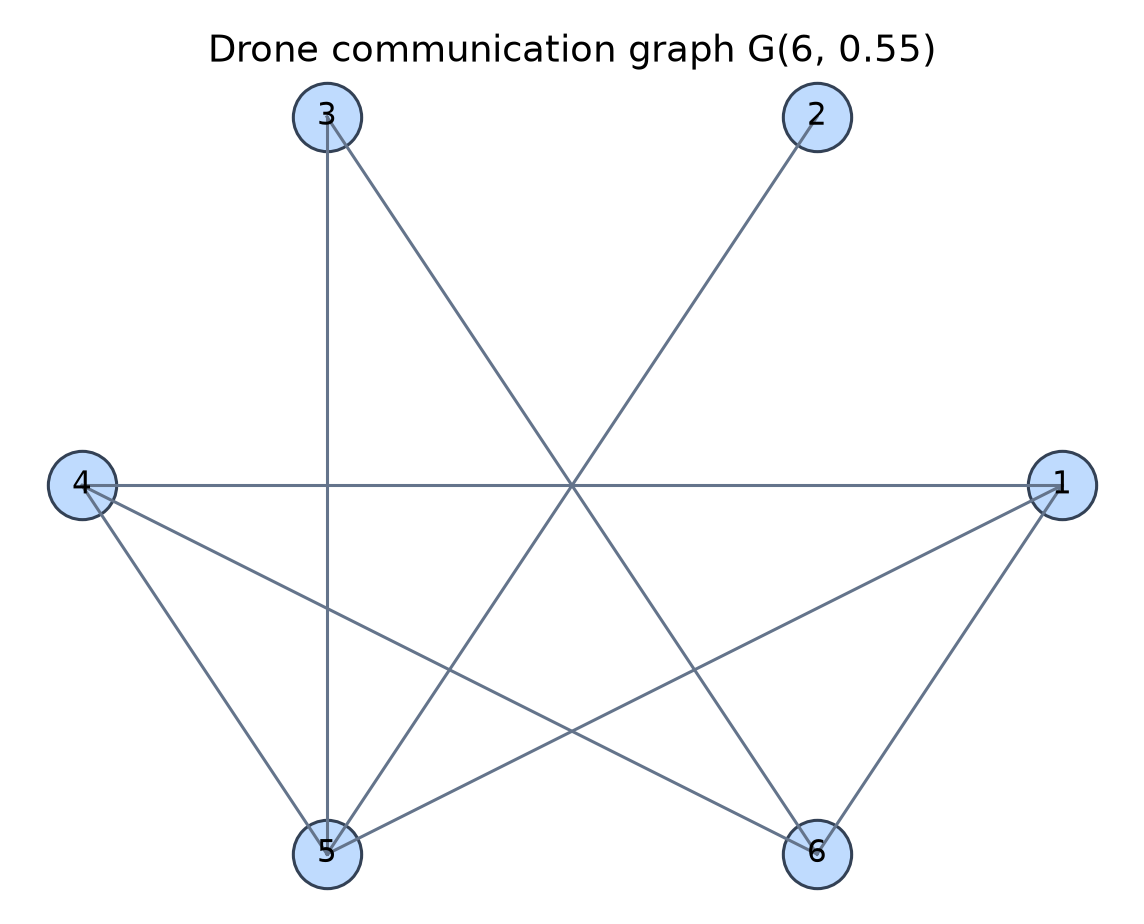
\includegraphics[width=.48\textwidth]{assets/p2_graph.png}
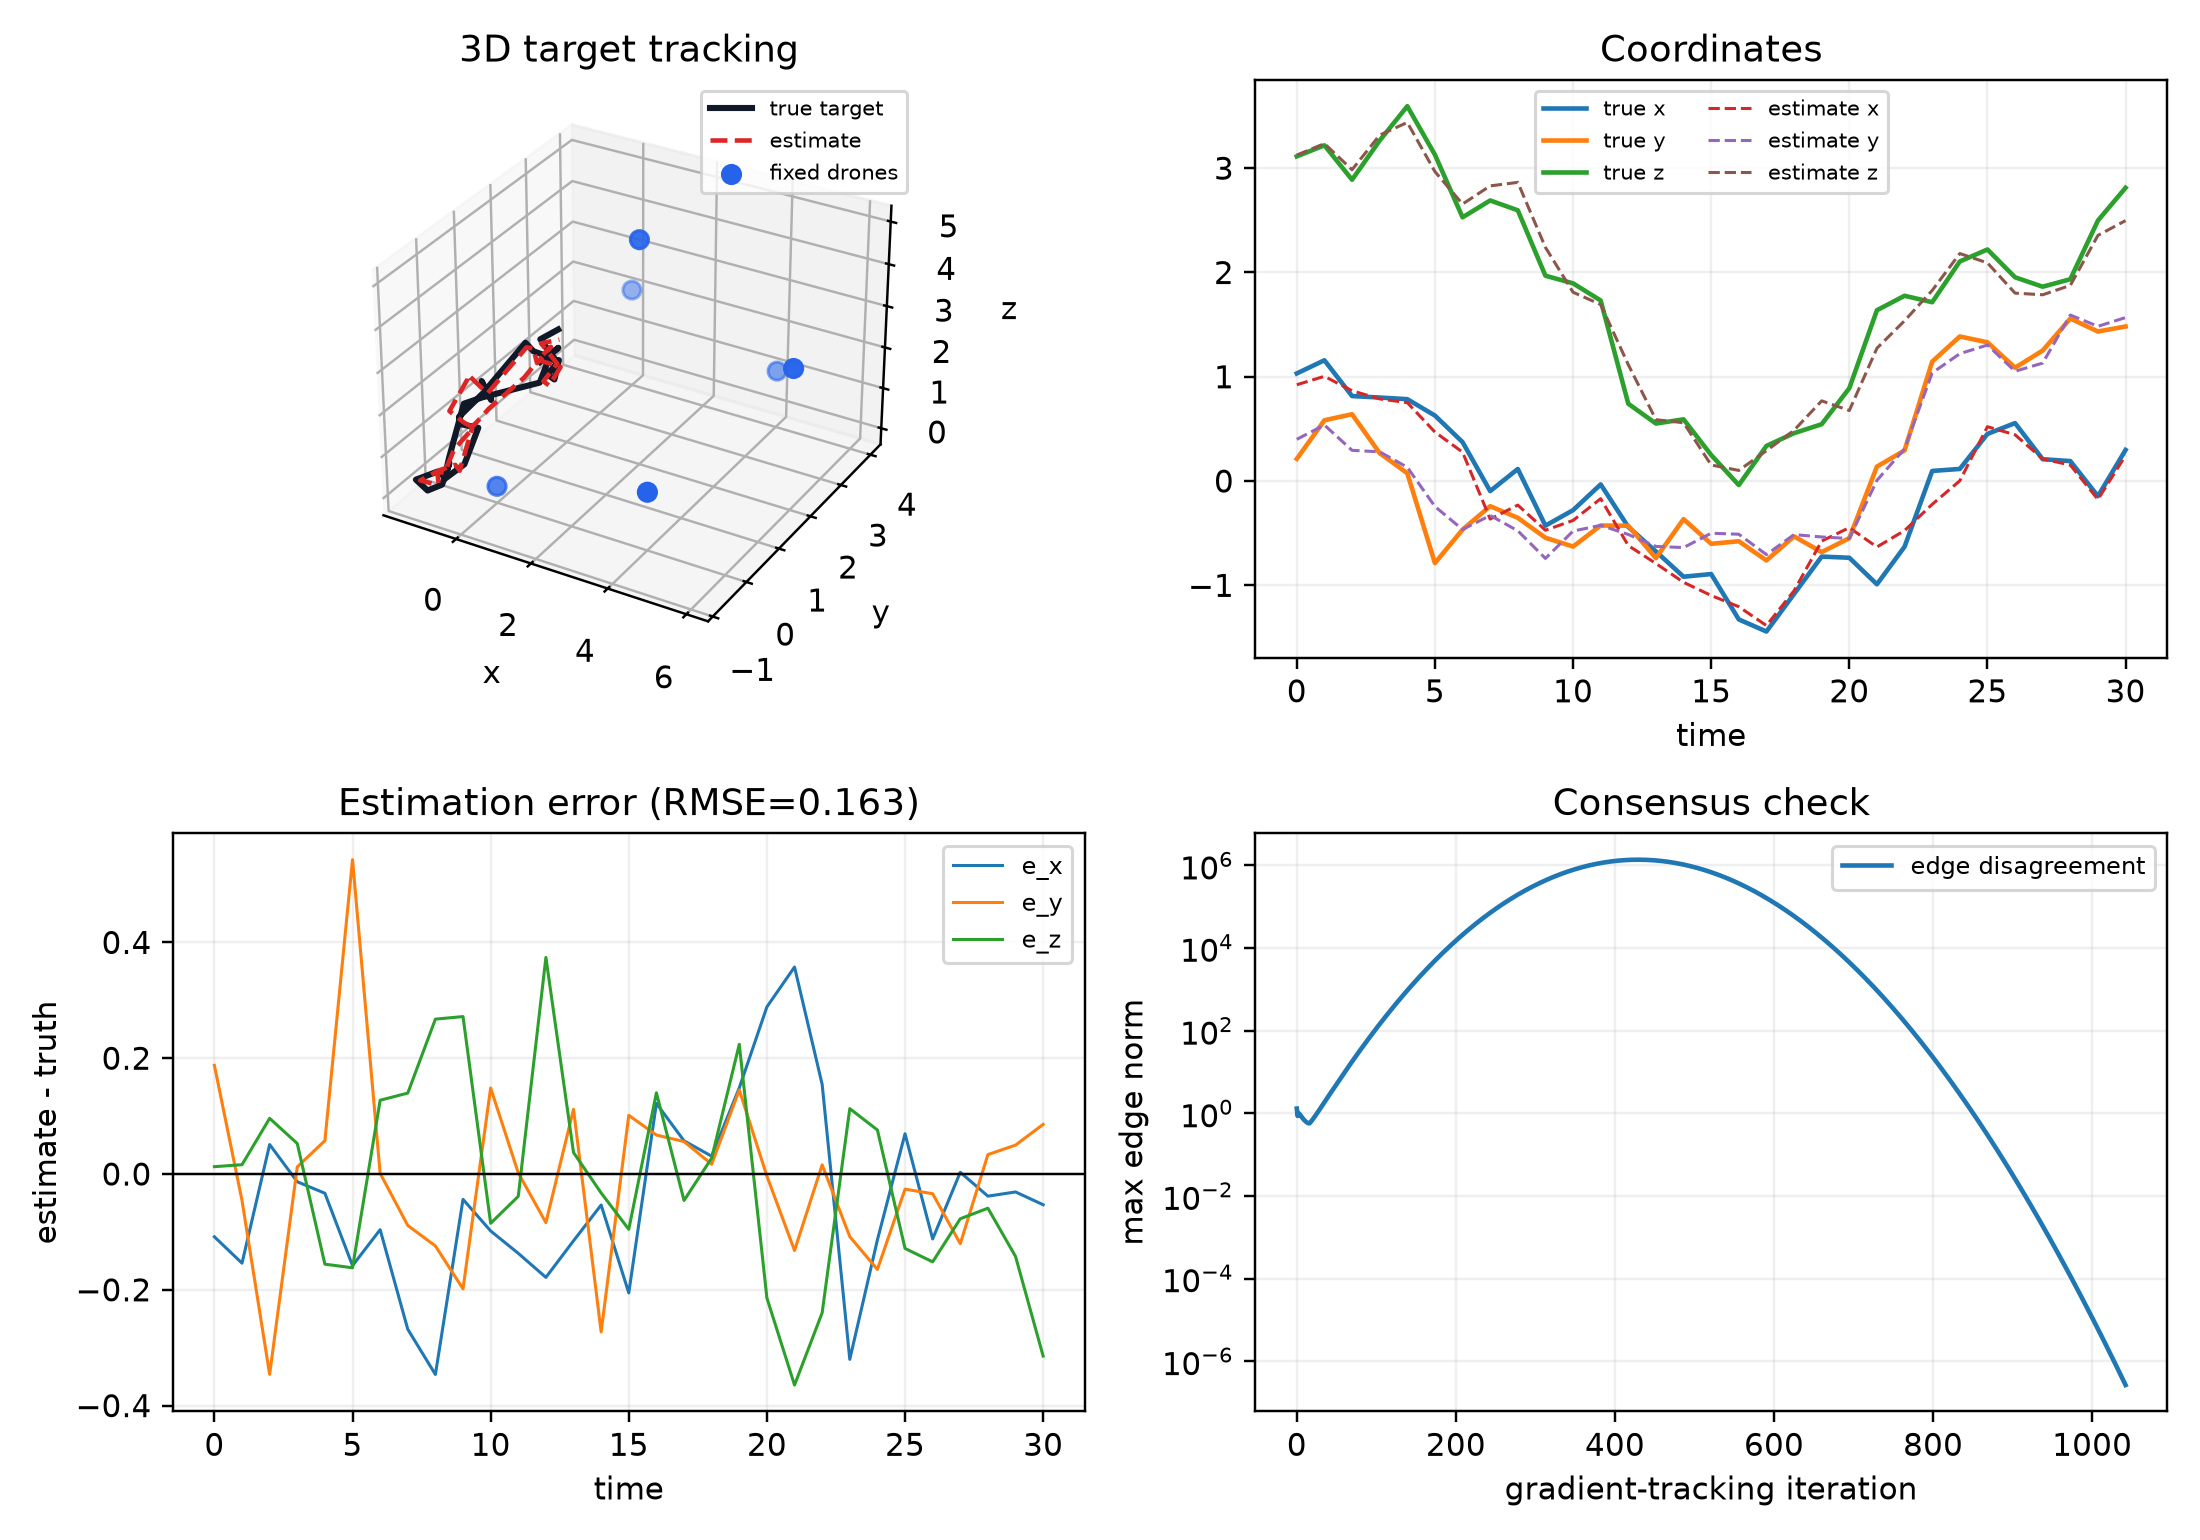
\includegraphics[width=.50\textwidth]{assets/p2_tracking_results.png}
\caption{Drone graph and the true/estimated target path, coordinate errors, and consensus check.}
\end{figure}

\subsection*{2.3 Numerical settings and result}
\[
\bar z_0=(2,-1,3)^\top,\quad
\Sigma_0=\operatorname{diag}(0.8,0.8,0.6),\quad
\Sigma_w=\operatorname{diag}(0.12,0.10,0.16).
\]
The fixed drone locations are
\[
\begin{bmatrix}0&0&0\\4&0&1\\0&4&2\\4&4&1\\2&2&5\\6&2&3\end{bmatrix}.
\]
The sensor covariance for drone $i$ is $(1+0.1i)\operatorname{diag}(0.22,0.20,0.28)$ with
$i=0,\ldots,5$. The corresponding mixing matrix is
\[
W=\begin{bmatrix}
.30&0&0&.25&.20&.25\\0&.80&0&0&.20&0\\0&0&.55&0&.20&.25\\
.25&0&0&.30&.20&.25\\.20&.20&.20&.20&.20&0\\.25&0&.25&.25&0&.25
\end{bmatrix},
\]
whose row and column sums are one. The final run used 1043 iterations. The final edge disagreement
was $2.64\times10^{-7}$ and the trajectory RMSE was $0.162559$. The estimate begins at
$(0.9233,0.4000,3.1256)$ and ends at $(0.2448,1.5676,2.4973)$.

The estimate follows the true trajectory closely in all three coordinates. The error plot provides
the clearest check: its three curves stay close to zero, and the RMSE is small compared with the
target's motion. The convergence panel records edge disagreement, while the stopping rule also
checks objective change. The graph and sensor locations remain fixed throughout the simulation.

\subsection*{Problem 2 code}
\lstinputlisting{Assignment_3_Problem_2.py}
\end{solution}

\clearpage
\begin{problem}{3}
There are $N\in\N$ agents connected via an undirected connected graph $G(V,E)$. They must
collaboratively execute $M\in\N$ tasks where $M>N$. The set of all tasks is denoted by
$\mathcal T:=\{T_1,\ldots,T_M\}$. Each agent $i\in V$ is assigned a local cost $C_{ij}$ for
performing a task $T_j\in\mathcal T$ and thereby giving us a cost matrix $C\in\R^{N\times M}$.
Further, each agent $i\in V$ has a capacity constraint $b_i\in\mathbb Z_{\ge0}$ which captures
how many tasks that agent can take. Since there are totally $M$ tasks and each task should be
assigned only once, $\sum_{i=1}^N b_i=M$. Do the following:
\begin{enumerate}
\item Formulate the task allocation problem as an optimization problem with appropriate cost
function and constraints. Your understanding of the problem and the way you formulate should be
highlighted well. Give the ADMM updates for every agent $i\in V$. The result should be a binary
linear program, which is NP-hard to solve for large $M,N$. Hence, you will need to do convex
relaxation.
\item Randomly choose the number of tasks $M$ and number of agents $N$ such that $M>N$. Fix them
and generate an undirected connected graph $G(V,E)$ for the communication model (use Erdos-Renyi
model). Randomly choose and fix the capacities $b_i$ for every agent such that $\sum_i b_i=M$.
Generate a random cost matrix $C\in\R^{N\times M}$ and ensure each element $C_{ij}>0$. Plot the
graph $G(V,E)$ and the result of task allocation using ADMM simulation. Fix the same $(M,N)$,
play with different generated cost matrices $C$ and plot the resulting task allocation and explain
your observations.
\end{enumerate}
\end{problem}

\begin{solution}
I choose $N=4$ agents and $M=7$ tasks, so $M>N$. The capacities are
$b=(2,2,2,1)$ and sum to 7. The connected graph uses $p=0.70$ and graph seed $20260906$;
its edges are $(1,2),(2,3),(2,4),(3,4)$. The three positive cost matrices use the same dimensions
and are generated successively from the fixed NumPy seed $20260905$.

\textbf{Complexity note.} With only the row-capacity, one-owner-per-task, and binary constraints
shown in the question, this is a capacitated transportation (min-cost-flow) problem. Its integral
row and column totals give an integral LP relaxation, so it is not generally NP-hard in this exact
form. I solve the stated model without adding a rounding step. The NP-hard hint in the question
would require additional constraints or a different allocation model.

\subsection*{3.1 Integer model and convex relaxation}
Let $x_{ij}=1$ if agent $i$ performs task $T_j$, and $x_{ij}=0$ otherwise. With
$X=[x_{ij}]\in\{0,1\}^{N\times M}$, the integer problem is
\[
\begin{aligned}
\min_X\quad &\langle C,X\rangle=\sum_{i=1}^N\sum_{j=1}^M C_{ij}x_{ij}\\
\text{subject to}\quad &\sum_{i=1}^N x_{ij}=1,\quad j=1,\ldots,M,\\
&\sum_{j=1}^M x_{ij}=b_i,\quad i=1,\ldots,N,\\
&x_{ij}\in\{0,1\}.
\end{aligned}
\]
The column constraint gives every task exactly one owner. The row constraint limits each agent to
its capacity, while the binary constraint prevents a task from being split between agents.

I relax the last constraint to $0\le x_{ij}\le1$. Because this is a transportation problem with
integer row and column totals, an optimum of the relaxed problem is integral. I still check this
numerically before displaying the final binary matrix.

\subsection*{3.2 ADMM splitting and updates}
For the numerical reference implementation, agent $i$ keeps the row $x_i\in\R^M$ and a
coordination copy $Z_{i,:}\in\R^M$. The matrix $Z$ is maintained by a coordinator in this
implementation; therefore the updates below are consensus-constrained ADMM updates, not a claim of
peer-to-peer ADMM over the plotted graph. Define
\[
\mathcal X_i=\{x_i\in[0,1]^M:\ones^\top x_i=b_i\},\qquad
\mathcal Z=\{Z\in[0,1]^{N\times M}:\ones^\top Z_{:j}=1\ \forall j\}.
\]
The relaxed problem is
\[
\min_{X,Z}\sum_{i=1}^N\left(C_i^\top x_i+I_{\mathcal X_i}(x_i)\right)+I_{\mathcal Z}(Z)
\quad\text{subject to }X-Z=0.
\]
Here $I_{\mathcal S}$ is zero on $\mathcal S$ and infinite outside it. With scaled dual matrix
$U\in\R^{N\times M}$ and penalty $\rho>0$, the updates are
\[
\begin{aligned}
x_i^{k+1}&=\argmin_{x_i\in\mathcal X_i}\left\{C_i^\top x_i+\frac\rho2\norm{x_i-z_i^k+u_i^k}_2^2\right\},\\
Z^{k+1}&=\argmin_{Z\in\mathcal Z}\frac\rho2\norm{X^{k+1}-Z+U^k}_F^2,\\
U^{k+1}&=U^k+X^{k+1}-Z^{k+1}.
\end{aligned}
\]
The first step is a local row problem. The second step adjusts each task column so that its entries
are nonnegative and sum to one; this is how the agents agree on task ownership. The graph is used
for the communication setting and connectivity check, but the central $Z$ projection is not a
peer-to-peer message-passing step.

For completeness, a genuine peer-to-peer version would give every node $i$ a full local copy
$X_i^{\mathrm{loc}}\in\R^{N\times M}$ and use
\[
\mathcal C_i=\left\{Y\in[0,1]^{N\times M}:\ones^\top Y_{:,j}=1\ \forall j,\quad
\ones^\top Y_{i,:}=b_i\right\}.
\]
For each undirected edge $(i,j)$ it would introduce an edge copy $Y_{ij}$ and impose the two
consensus constraints $X_i^{\mathrm{loc}}=Y_{ij}$ and $X_j^{\mathrm{loc}}=Y_{ij}$. With oriented
scaled duals $U_{ij}$ and $U_{ji}$, the edge-wise updates are
\[
\begin{aligned}
X_i^{k+1}&=\argmin_{Y\in\mathcal C_i}\left\{C_{i,:}Y_{i,:}^{\top}
 +\frac{\rho}{2}\sum_{j\in\mathcal N_i}\|Y-Y_{ij}^k+U_{ij}^k\|_F^2\right\},\\
Y_{ij}^{k+1}&=\tfrac12\left(X_i^{k+1}+U_{ij}^k+X_j^{k+1}+U_{ji}^k\right),\\
U_{ij}^{k+1}&=U_{ij}^k+X_i^{k+1}-Y_{ij}^{k+1}.
\end{aligned}
\]
The last dual update is run at both ends of every edge. Node $i$ sends $X_i^{k+1}$ only to its
neighbours, and each edge forms its average from the two received copies. This is the proper
peer-to-peer formulation, but the figures below use the simpler coordinator-based reference solver.

Both projections use the same simple rule. For a vector $v$, the projection onto
$\{q:0\le q\le1,\ones^\top q=b\}$ is
\[
\Pi_b(v)=\operatorname{clip}(v-\theta,0,1),
\]
where the scalar $\theta$ is chosen so that the entries sum to $b$. Thus the row update applies
this rule to $z_i^k-u_i^k-C_i/\rho$, and the column update applies it to $X_{:j}^{k+1}+U_{:j}^k$
with $b=1$.

\subsection*{3.3 Simulation and results}
I use $\rho=1$, primal and dual tolerances $10^{-5}$, and at most 12000 iterations. The ADMM
residuals are $r^k=X^k-Z^k$ and $s^k=\rho(Z^k-Z^{k-1})$. All three runs reached both tolerances,
and all relaxed solutions were integral up to $2\times10^{-4}$; no rounding or repair was needed.

\begin{figure}[H]
\centering
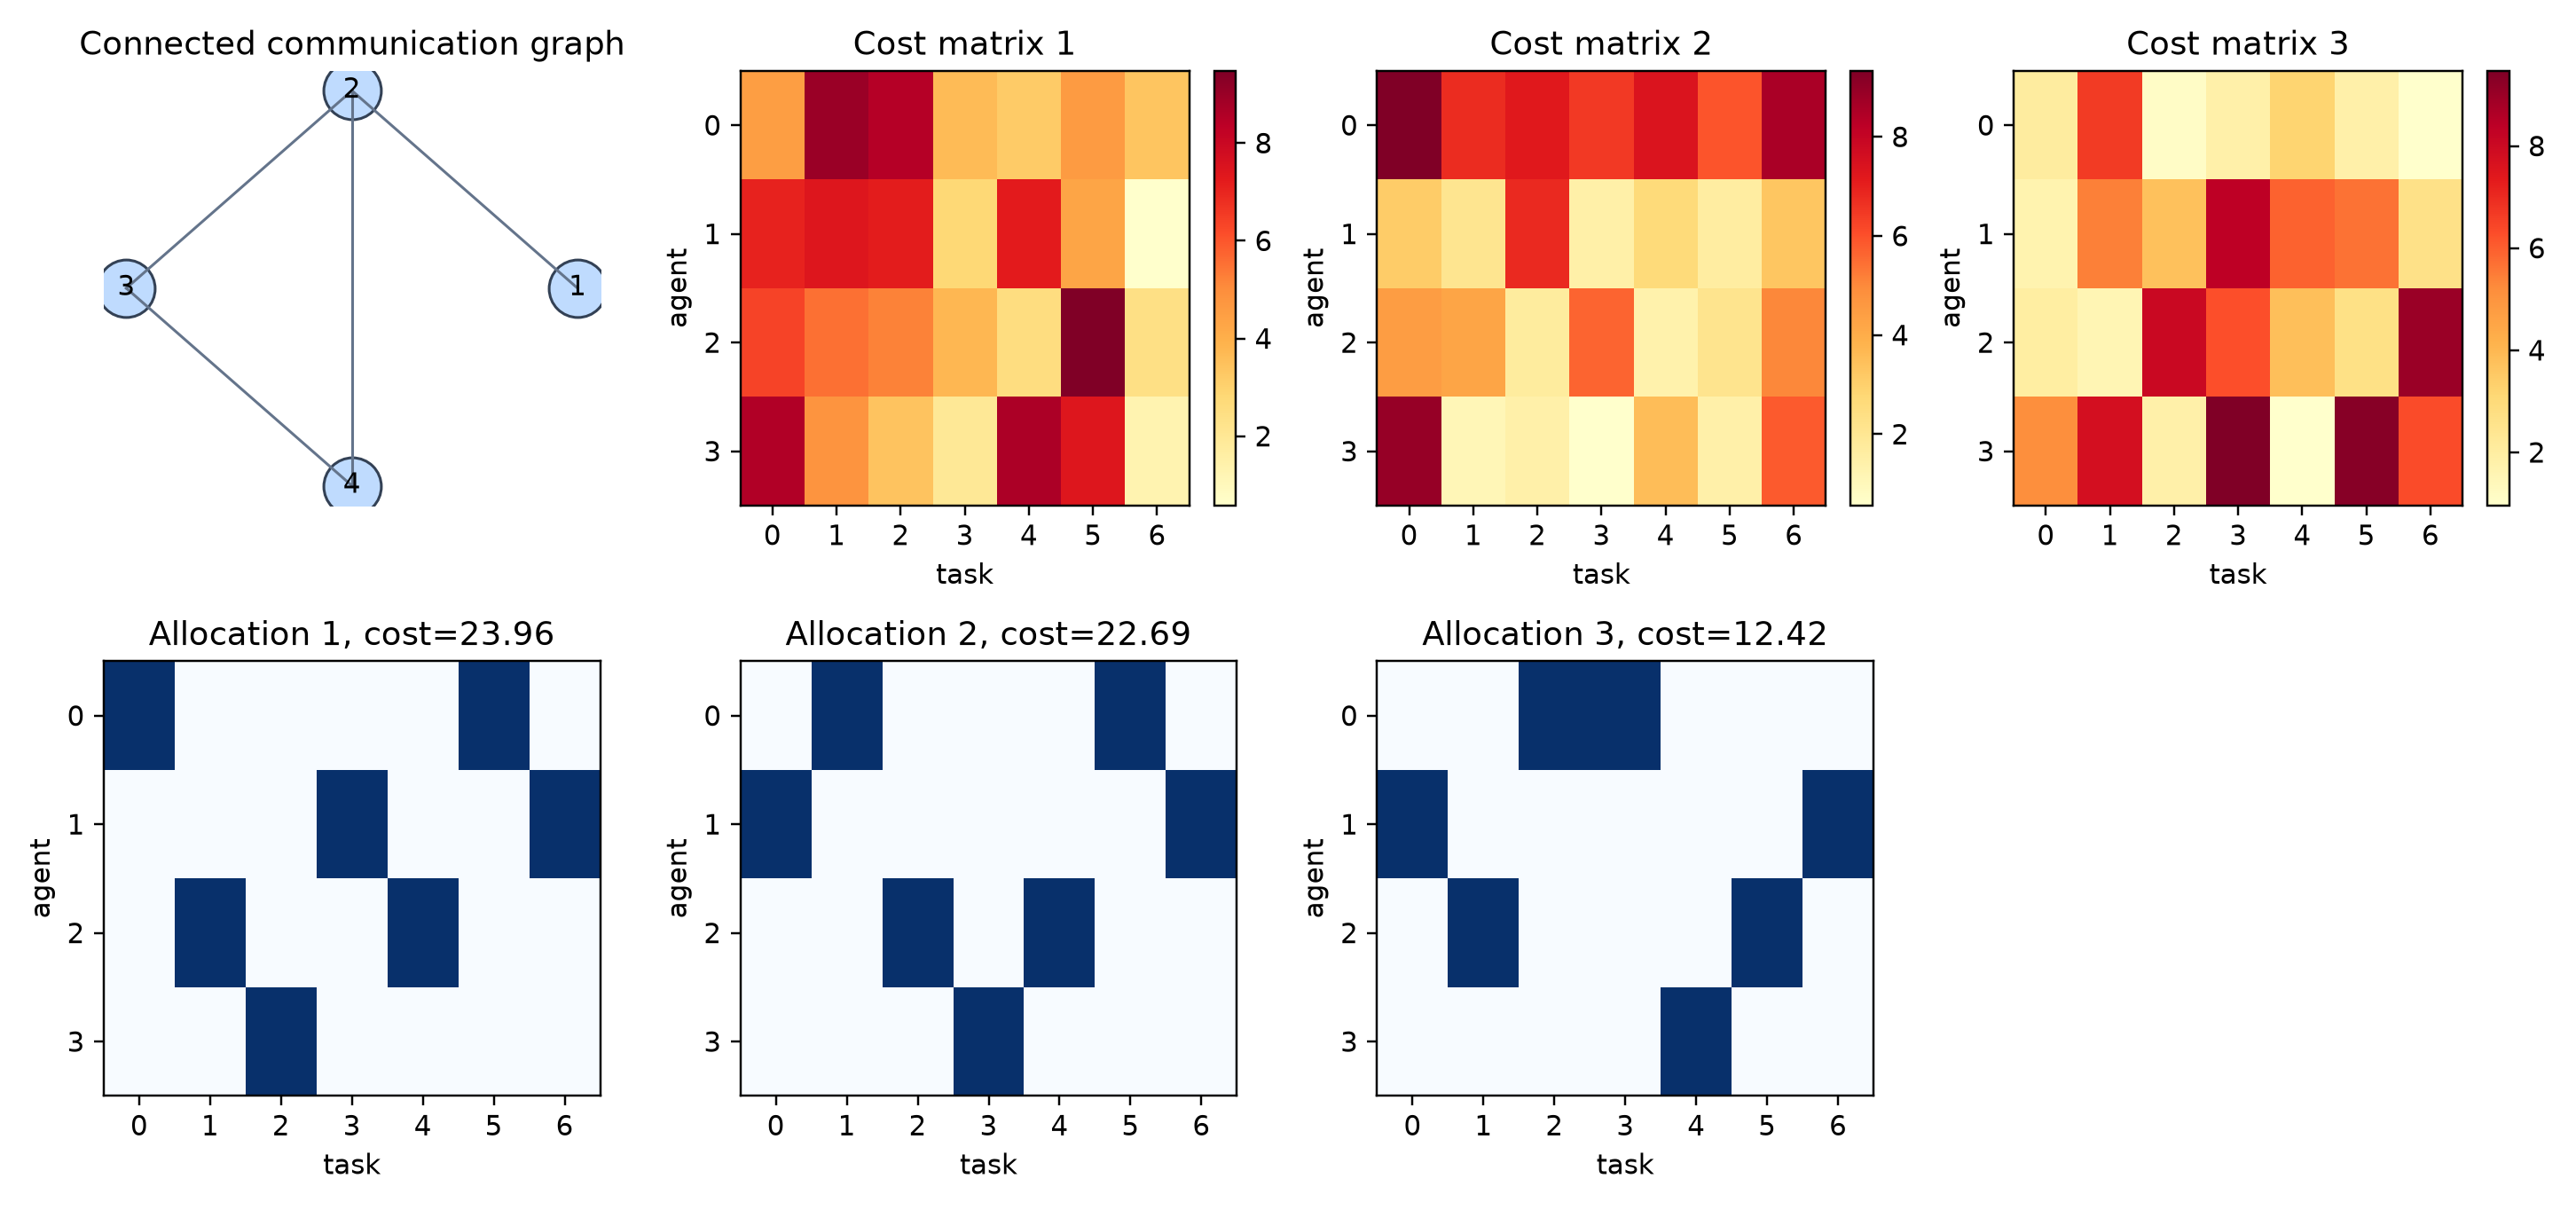
\includegraphics[width=.98\textwidth]{assets/p3_allocation_results.png}
\caption{Communication graph, positive cost heatmaps, and the three binary task allocations.}
\end{figure}

\begin{center}
\small
\begin{tabular}{@{}lrrrrrrr@{}}
\toprule
case & iters & $\|r\|$ & $\|s\|$ & total cost & row & column & changed\\
\midrule
baseline & 9 & $5.44\times10^{-16}$ & $0$ & 23.962868 & pass & pass & 0\\
case 2 & 11 & $5.21\times10^{-16}$ & $4.97\times10^{-16}$ & 22.693173 & pass & pass & 4\\
case 3 & 6 & $5.33\times10^{-16}$ & $2.54\times10^{-16}$ & 12.415220 & pass & pass & 5\\
\bottomrule
\end{tabular}
\end{center}

The three displayed binary allocation matrices are
\[
\begin{array}{c@{\qquad}c@{\qquad}c}
X^{(1)}=\begin{bmatrix}1&0&0&0&0&1&0\\0&0&0&1&0&0&1\\0&1&0&0&1&0&0\\0&0&1&0&0&0&0\end{bmatrix}&
X^{(2)}=\begin{bmatrix}0&1&0&0&0&1&0\\1&0&0&0&0&0&1\\0&0&1&0&1&0&0\\0&0&0&1&0&0&0\end{bmatrix}&
X^{(3)}=\begin{bmatrix}0&0&1&1&0&0&0\\1&0&0&0&0&0&1\\0&1&0&0&0&1&0\\0&0&0&0&1&0&0\end{bmatrix}.
\end{array}
\]
Each matrix has column sums equal to one and row sums equal to $(2,2,2,1)$.

\begin{figure}[H]
\centering
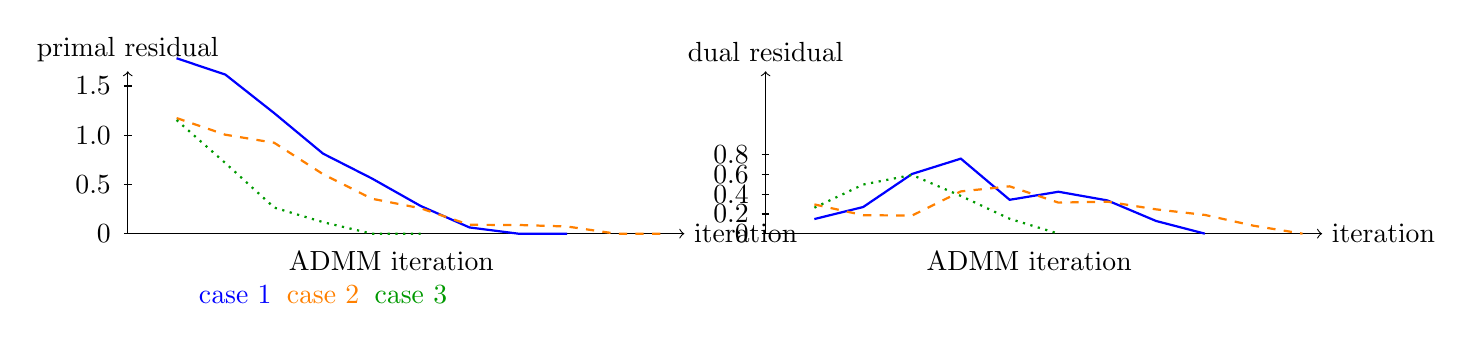
\begin{tikzpicture}[x=0.62cm,y=1.25cm]
\begin{scope}
\draw[->] (0,0) -- (11.4,0) node[right] {iteration};
\draw[->] (0,0) -- (0,1.65) node[above] {primal residual};
\foreach \y/\lab in {0/0,0.5/0.5,1/1.0,1.5/1.5}{\draw (-0.08,\y) -- (0.08,\y) node[left=4pt] {\lab};}
\draw[blue,thick] plot coordinates {(1,1.7824)(2,1.6160)(3,1.2247)(4,.8134)(5,.5612)(6,.2814)(7,.0632)(8,0)(9,0)};
\draw[orange,thick,dashed] plot coordinates {(1,1.1746)(2,1.0053)(3,.9236)(4,.6046)(5,.3552)(6,.2580)(7,.0899)(8,.0884)(9,.0729)(10,0)(11,0)};
\draw[green!60!black,thick,dotted] plot coordinates {(1,1.1544)(2,.7171)(3,.2650)(4,.1171)(5,0)(6,0)};
\node at (5.4,-0.28) {ADMM iteration};
\end{scope}
\begin{scope}[xshift=8.1cm]
\draw[->] (0,0) -- (11.4,0) node[right] {iteration};
\draw[->] (0,0) -- (0,1.65) node[above] {dual residual};
\foreach \y/\lab in {0/0,0.2/0.2,0.4/0.4,0.6/0.6,0.8/0.8}{\draw (-0.08,\y) -- (0.08,\y) node[left=4pt] {\lab};}
\draw[blue,thick] plot coordinates {(1,.1485)(2,.2709)(3,.6066)(4,.7623)(5,.3442)(6,.4260)(7,.3382)(8,.1289)(9,0)};
\draw[orange,thick,dashed] plot coordinates {(1,.2973)(2,.1877)(3,.1839)(4,.4294)(5,.4810)(6,.3154)(7,.3253)(8,.2470)(9,.1903)(10,.0805)(11,0)};
\draw[green!60!black,thick,dotted] plot coordinates {(1,.2637)(2,.4992)(3,.5967)(4,.3835)(5,.1512)(6,0)};
\node at (5.4,-0.28) {ADMM iteration};
\end{scope}
\node[blue] at (2.2,-0.62) {case 1};\node[orange] at (4.0,-0.62) {case 2};\node[green!60!black] at (5.8,-0.62) {case 3};
\end{tikzpicture}
\caption{Primal and dual residual histories for the three fixed cost matrices.}
\end{figure}

The task-owner rows below list the owner of tasks $T_1$ through $T_7$:
\[
\begin{array}{c|ccccccc}
\text{baseline}&1&3&4&2&3&1&2\\
\text{case 2}&2&1&3&4&3&1&2\\
\text{case 3}&2&3&1&1&4&3&2
\end{array}
\]
The baseline assignment gives two tasks to agents 1, 2, and 3, and one to agent 4. Every column
has one owner and the row counts are $(2,2,2,1)$. With a new cost matrix, task preferences change,
so the capacity limits can move tasks even when an agent has a low cost for them. The changes are
therefore explained by the new costs and capacity limits, not by random behaviour.

\subsection*{Problem 3 code}
\lstinputlisting{Assignment_3_Problem_3.py}
\end{solution}

\clearpage
\begin{problem}{4}
Consider the LASSO problem
\[
\min_x\left[\frac12\norm{Ax-b}_2^2+\lambda\norm{x}_1\right].
\]
Write the ADMM iteration updates by solving and writing the closed form solution for $x,z$ updates.
\end{problem}

\begin{solution}
Assume $A\in\R^{m\times n}$, $b\in\R^m$, $x,z\in\R^n$, $\lambda\ge0$, and $\rho>0$.
Introduce $z$ and impose $x-z=0$:
\[
\min_{x,z}\ \frac12\norm{Ax-b}_2^2+\lambda\norm{z}_1
\quad\text{subject to }x-z=0.
\]
This split keeps the least-squares term with $x$ and the absolute-value penalty with $z$.

Using the scaled dual variable $u$ and penalty $\rho>0$, the scaled augmented Lagrangian is
\[
\mathcal L_\rho(x,z,u)=\frac12\norm{Ax-b}_2^2+\lambda\norm{z}_1
 +\frac\rho2\norm{x-z+u}_2^2-\frac\rho2\norm{u}_2^2.
\]

\subsection*{4.1 The $x$ update}
Holding $z^k$ and $u^k$ fixed, minimise the smooth part. Its gradient is
\[
A^\top(Ax-b)+\rho(x-z^k+u^k).
\]
Setting it to zero gives the normal equation
\[
(A^\top A+\rho I)x^{k+1}=A^\top b+\rho(z^k-u^k).
\]
Since $A^\top A$ is positive semidefinite and $\rho I$ is positive definite,
$A^\top A+\rho I$ is invertible. Hence the closed form is
\[
\boxed{x^{k+1}=(A^\top A+\rho I)^{-1}\left(A^\top b+\rho(z^k-u^k)\right).}
\]
In implementation, solve this linear system directly instead of computing the matrix inverse.

\subsection*{4.2 The $z$ update}
Set $v=x^{k+1}+u^k$. The $z$ subproblem is
\[
z^{k+1}=\argmin_z\left\{\lambda\norm{z}_1+\frac\rho2\norm{z-v}_2^2\right\}.
\]
It separates over coordinates. For one coordinate, minimise
$\lambda|z_j|+\frac\rho2(z_j-v_j)^2$. The three cases are:
\[
z_j=\begin{cases}
v_j-\lambda/\rho,&v_j>\lambda/\rho,\\
0,&|v_j|\le\lambda/\rho,\\
v_j+\lambda/\rho,&v_j<-\lambda/\rho.
\end{cases}
\]
Therefore the closed form is the soft-threshold operation
\[
\boxed{z^{k+1}=S_{\lambda/\rho}(x^{k+1}+u^k)},\qquad
[S_\kappa(v)]_j=\operatorname{sign}(v_j)\max\{|v_j|-\kappa,0\}.
\]
In simple terms: small entries become zero, while larger entries move toward zero.

\subsection*{4.3 Dual update and complete iteration}
The scaled dual update is
\[
\boxed{u^{k+1}=u^k+x^{k+1}-z^{k+1}.}
\]
The quantity $x^{k+1}-z^{k+1}$ is the primal feasibility residual. Thus one complete ADMM
iteration is the linear solve for $x$, soft thresholding for $z$, and the dual update above.

\end{solution}

\section*{AI-use declaration}
I used AI assistance only to improve the final writing of this assignment.

\end{document}
